\section{ФУНКЦИОНАЛЬНОЕ ПРОЕКТИРОВАНИЕ}
\label{sec:func}

Разработка функционала программного обеспечения является целью 
функционального проектирования. Алгоритм работы модуля представлен на чертеже \blockScheme.

В данном разделе модули описаны с точки зрения разработки функций, которые реализуются в
дипломном проекте. Функциональное проектирование нацелено на создание корректно и
эффективно работающего проекта. Представление необходимого функционала~-- основная задача текущего раздела. После анализа требуемых для реализации программного продукта
функций, было решено разбить программу на следующие модули:

\begin{itemize}
    \item блок первичной обработки;
    \item блок автоматической сегментации;
    \item блок обработки текста;
    \item блок сегментации по точкам;
    \item блок обработки маски;
    \item блок обработки данных для диффузионной модели;
    \item блок работы диффузионной модели для генерации изображение;
    \item блок графического интерфейса.
\end{itemize}

\subsection{Блок графического интерфейса}

Данный блок представляет собой набор методов, которые является частью пользовательского интерфейса, которые обеспечивает взаимодействие пользователя с модулем. Данный блок ориентирован сугубо на пользователя, предоставляет все необходимые инструменты для эффективной работы с модулем, делая процесс более интуитивно понятным и доступным. Это облегчает взаимодействие, управление и анализ, повышая удобство использования и функциональность системы в целом.

Метод \lstinline{create_widgets} создаёт интерактивные виджеты для управления параметрами и выбора изображений в процессе работы с диффузионной моделью. Параметры:

\begin{itemize}
    \item \lstinline{original_image_filename}~-- имя файла оригинального изображения, которое используется для восстановления в случае выбора его из виджета \lstinline{dropdown};
    \item \lstinline{inpainted_images_pathes}~-- список путей к изменённым изображениям, которые можно выбрать и отобразить через виджет \lstinline{dropdown}.
\end{itemize}

Виджеты для управления:

\begin{itemize}
    \item \lstinline{quality_control_slider}~-- cлайдер для управления качеством генерируемых изображений. Этот параметр может варьироваться от минимального до максимального значения качества, влияя на разрешение и четкость конечного изображения. Он позволит пользователям выбирать между более высоким качеством изображения и меньшим временем генерации;
    \item \lstinline{num_images_per_prompt_slider}~-- cлайдер для выбора количества изображений, генерируемых за один запрос;
    \item \lstinline{guidance_scale_widget}~-- виджет для ввод числа для масштаба направляющих, который влияет на степень детализации в генерируемых изображениях;
    \item \lstinline{image_rotation_widget}~-- виджет для вращения изображения, позволяющий задать угол поворота изображения перед обработкой. Это может быть полезно для корректировки ориентации изображения или для экспериментов с разными перспективами;
    \item \lstinline{brightness_control_slider}~-- слайдер для регулировки яркости генерируемых изображений. Это позволит пользователю изменять освещенность изображения, что может быть особенно полезно при работе с изображениями в разных световых условиях.
    \item \lstinline{contrast_control_slider}~-- слайдер для управления контрастом изображения. Увеличение или уменьшение контраста может значительно изменить визуальное восприятие и эстетическую ценность изображений.
    \item \lstinline{num_inference_steps_widget}~-- ввод числа для количества шагов инференции, определяющий, как много итераций модель выполнит перед финализацией изображения.
\end{itemize}

\lstinline{Dropdown} для выбора изображений:

\begin{itemize}
    \item \lstinline{inpainted_img_to_select_dropdown}~-- дропдаун для выбора изображения из списка доступных оригинальных и обработанных изображений.
    \item \lstinline{color_variation_dropdown}~-- выпадающий список для выбора предпочтительной цветовой палитры или стиля изображения. Это может включать опции, такие как <<Яркие цвета>>, <<Пастельные тона>>, <<Черно-белый>>. Пользователи могут использовать этот параметр для управления общим визуальным стилем генерируемых изображений;
    \item \lstinline{texture_style_dropdown}~-- выпадающий список для выбора стиля текстуры изображения, который может включать варианты, такие как <<Гладкий>>, <<Текстурированный>>, <<Холст>>. Это позволит пользователям вносить изменения в визуальное восприятие материалов на изображении.
\end{itemize}

Кнопки для управления процессом:

\begin{itemize}
    \item \lstinline{btn_next}~-- кнопка для продолжения работы, применяющая выбранные параметры и переходящая к следующему шагу обработки;
    \item \lstinline{btn_quit}~-- кнопка для остановки процесса и сохранения текущего состояния;
    \item \lstinline{reset_button}~-- Кнопка для сброса всех виджетов и параметров к исходным значениям. Это удобно, когда пользователи хотят начать процесс заново без необходимости вручную возвращать каждый параметр в исходное положение.
\end{itemize}

Внутренние функции:
\begin{itemize}
    \item \lstinline{make_options_dropdown}~-- функция для создания опций выпадающего списка, которая генерирует пары значений (название изображения, индекс) для каждого изображения. Это позволяет пользователю выбирать из различных версий обработанных изображений для просмотра и дальнейших действий;
    \item \lstinline{get_selected_image_name}~-- вспомогательная функция, которая определяет имя файла выбранного изображения на основе текущего значения выпадающего списка. Это имя файла используется для загрузки и отображения изображения;
    \item \lstinline{on_btn_next_clicked}~-- обработчик клика на кнопку <<Продолжить>>, применяющий выбранные параметры и запускающий следующий шаг обработки;
    \item \lstinline{on_btn_quit_clicked}~-- обработчик клика на кнопку <<Остановить>>, сохраняющий текущее состояние и завершающий процесс.
\end{itemize}

Метод \lstinline{display_widgets} отображает все созданные виджеты в пользовательском интерфейсе. Он итерирует по списку \lstinline{self.widgets_ls}, который содержит все созданные виджеты, и отображает каждый из них с помощью функции \lstinline{display}, что делает виджеты видимыми и интерактивными для пользователя.

Метод \lstinline{paint_mask_on_img} реализует интерактивный интерфейс для ручной рисовки маски на изображении, который интегрирован с помощью JavaScript в веб-браузере. Метод позволяет пользователю вносить изменения в изображение, создавая маску, которая будет использована в процессе диффузии для изменения или улучшения изображения. Параметры:

\begin{itemize}
    \item \lstinline{img_filename}~-- имя файла изображения, на котором пользователь будет рисовать маску;
    \item \lstinline{quality}~-- качество изображения после сохранения изменений. Это вещественное число, определяющее степень сжатия изображения. Значение по умолчанию~-- 0.8.
\end{itemize}

Метод использует API JavaScript для создания интерактивных элементов HTML и интеграции их с текущей сессией Jupyter Notebook. Вот основные шаги работы метода:

\begin{enumerate_num}
    \item Cоздание элементов интерфейса. Создается текстовое поле для ввода комментариев о том, что пользователь желает нарисовать; Создается ползунок для выбора размера кисти; Добавляются кнопки для начала и завершения рисования.
    
    \item Настройка холста для рисования. Иинициализируется HTML-холст, который служит областью для рисования маски; Пользователь может рисовать на холсте, изменяя его содержимое в реальном времени.

    \item Обработка данных. Определяются обработчики событий для мыши, позволяющие пользователю рисовать на холсте путем перемещения курсора при зажатой кнопке мыши; Реализуется функция, которая собирает данные с холста после завершения рисования и преобразует их в формат данных изображения, которые можно дальше используются в коде.

    \item Завершение рисования. После того как пользователь завершает рисование и нажимает кнопку обработки, данные изображения и введенный текст отправляются обратно в Python для дальнейшей обработки или сохранения.
\end{enumerate_num}

Метод активно использует JavaScript для создания интерактивных элементов и обработки пользовательского ввода. JavaScript обеспечивает динамическое взаимодействие на стороне клиента, что делает процесс рисования маски более удобным и интуитивно понятным. Это включает в себя рисование на холсте, обработку ввода данных и передачу результатов обратно в Python.

Этот метод значительно улучшает взаимодействие пользователя с системой, позволяя прямо влиять на результаты обработки изображений через интерфейс рисования масок.

Методы обратной связи, такие как \lstinline{display_results} и \lstinline{log_status}, играют критическую роль в интерактивных системах и приложениях, поскольку они предоставляют пользователям необходимую информацию о статусе операций, результатах обработки и других важных аспектах работы системы. Эти методы могут помочь улучшить пользовательский опыт, обеспечивая своевременное и понятное представление данных и событий системы.

Метод \lstinline{display_results} предназначен для визуализации результатов работы модуля или системы. Он отображает графическую информацию, текстовые данные или комбинировать оба этих элемента в зависимости от типа данных и нужд пользователя. Параметры:

\begin{itemize}
    \item \lstinline{results}~-- данные или объекты, которые нужно визуализировать. Это могут быть изображения, текстовые сообщения о результате операций.
\end{itemize}

Метод \lstinline{log_status} предназначен для логирования различных событий и статусов системы, обеспечивая возможность отслеживать ход выполнения процессов и возможные ошибки. Параметры:

\begin{itemize}
    \item \lstinline{message}~-- текст сообщения, которое должно быть залогировано;
    \item \lstinline{level}~-- уровень важности сообщения.
\end{itemize}

Блок методов, ориентированный на пользователя, предоставляет все необходимые инструменты для эффективной работы с модулем, делая процесс более интуитивно понятным и доступным. Это облегчает взаимодействие, управление и анализ, повышая удобство использования и функциональность системы в целом. В дополнение к этому, пользовательские методы позволяют настраивать систему под конкретные задачи и предпочтения, обеспечивая интеграцию с  процессами.

\subsection{Блок автоматической сегментации}

В основе блока автоматический сегментации лежит класс \lstinline{Segmentation} который содержит в себе все необходимые методы для автоматической сегментации изображения. Класс представляет собой реализацию для работы с сегментацией изображений, используя предоставленную модель для генерации и обработки масок.

Конструктор \lstinline{__init__} инициализирует экземпляр класса, устанавливая начальные значения атрибутов для хранения пути к изображению, самого изображения, масок, а также модели и размеров изображения. Входные параметры:

\begin{itemize}
    \item \lstinline{model}~-- модель, для сегментации. Эта модель будет использоваться для генерации масок сегментации из изображений;
    \item \lstinline{image_path}~-- строка, указывающая путь к изображению, которое будет обрабатываться;
    \item \lstinline{image_resize}~-- кортеж из двух целых чисел, указывающий размеры, до которых должно быть изменено изображение перед обработкой. Это помогает нормализовать входные данные для модели.
\end{itemize}

Метод \lstinline{read_image} читает изображение из указанного пути, преобразует его цвета из BGR в RGB (стандартное представление цветов в OpenCV в BGR), и изменяет его размер. Возвращает обработанное изображение. Входные параметры:

\begin{itemize}
    \item \lstinline{image_path}~-- путь к файлу изображения, который нужно загрузить;
    \item \lstinline{image_resize}~-- кортеж, задающий размер изображения после изменения размера. Если передан \lstinline{None}, изменение размера не выполняется.
\end{itemize}

Метод \lstinline{predict} не принимает параметров. Он интегрирует несколько шагов для выполнения полного цикла сегментации:

\begin{enumerate_num}
    \item Считывает и подготавливает изображение.
    \item Генерирует маски сегментации для этого изображения.
    \item Выбирает и расширяет маски с помощью внутренних методов класса.
    \item Возвращает подготовленные маски для дальнейшего использования.
\end{enumerate_num}

Метод \lstinline{_get_masks} не принимает параметров. Активирует модель на GPU, использует объект генератора масок для создания масок из текущего изображения. Возвращает сгенерированные маски, каждой из которых присваивается уникальный индекс. Далее показан подробные алгоритм работы: 

\begin{enumerate_num}
    \item Активирует модель на GPU.
    \item Использует созданный генератор масок для изображения.
    \item Добавляет индекс каждой маске для последующего использования.
    \item Возвращает список сгенерированных масок.
\end{enumerate_num}

Метод \lstinline{masks_selection} не принимает параметров. Вызывает статический метод \lstinline{_auto_masks_selection}, который автоматически выбирает подходящие маски из списка сгенерированных. Возвращает подготовленные маски.

Метод \lstinline{get_intersection} возвращает количество пересекающихся пикселей между двумя масками, что может используется для определения степени перекрытия между двумя сегментами. Входные параметры:

\begin{itemize}
    \item \lstinline{mask_id_1}~-- индекс первой маски;
    \item \lstinline{mask_id_2}~-- индекс второй маски.
\end{itemize}

Метод \lstinline{join_masks} объединяет маски по указанным индексам, возвращая результат как единую маску. Если \lstinline{mask_id_1} является списком, объединяет все маски в этом списке. Входные параметры:

\begin{itemize}
    \item \lstinline{mask_id_1}~-- индекс первой маски; 
    \item \lstinline{mask_id_2}~-- индекс второй маски (опционально).
\end{itemize}

Метод \lstinline{get_mask_by_id} возвращает маску по её индексу. Возвращает маску в виде массива данных. Входные параметры:

\begin{itemize}
    \item \lstinline{mask_id}~-- индекс маски.
\end{itemize}

Метод \lstinline{get_main_masks} возвращает список <<главных>> масок, предварительно подготовленных масок и возвращает их.

Метод \lstinline{get_inner_masks} возвращает все <<внутренние>> или <<дочерние>> маски, связанные с указанной главной маской. Входные параметры:

\begin{itemize}
    \item \lstinline{idx}~-- индекс главной маски.
\end{itemize}

Метод \lstinline{expand_masks} расширяет и организует выбранные маски в более удобную для использования структуру данных. Этот метод позволяет структурированно сохранить иерархические связи между масками, что упрощает последующий доступ и манипуляции с масками в зависимости от их взаимосвязей. Входные параметры:

\begin{itemize}
    \item \lstinline{masks}~-- список кортежей, где каждый кортеж содержит два элемента: индекс основной маски и список кортежей дочерних масок.
\end{itemize}

Метод \lstinline{_auto_masks_selection} автоматически выбирает наиболее подходящие маски из предоставленного списка сгенерированных масок. Этот метод обеспечивает автоматический и эффективный отбор и организацию масок, что критически важно для упрощения последующей обработки изображений в задачах сегментации. Входные параметры:

\begin{itemize}
    \item \lstinline{masks}~-- cписок масок, где каждая маска представлена словарем с ключами, такими как \lstinline{idx} (уникальный индекс маски) и  \lstinline{segmentation} (массив маски сегментации).
\end{itemize}

\subsection{Блок сегментации по точкам}

Класс \lstinline{SegmentationByPoints} предоставляет функционал для сегментации изображений на основе интерактивного выбора точек пользователем. Эти точки могут быть как положительными (позитивные координаты), так и отрицательными (негативные координаты), что позволяет модели более точно определить области изображения для сегментации.

Конструктор \lstinline{__init__} инициализирует экземпляр класса с начальными параметрами. Он сохраняет путь к изображению и создаёт экземпляр модели сегментации, предназначенной для последующего использования при генерации масок. Помимо этого, инициализируются переменные для хранения изображения, координат выбранных точек и финальной маски. Параметры:

\begin{itemize}
    \item \lstinline{image_path}~-- cтрока, содержащая путь к изображению для сегментации.
\end{itemize}

Метод \lstinline{read_image} не принимает параметров. Он загружает изображение из файла, указанного в \lstinline{image_path}, используя библиотеку Matplotlib для чтения и OpenCV для изменения размера изображения до унифицированного размера (512x512 пикселей).

Метод \lstinline{predict_mask} не принимает параметров. Он утверждает, что выбор точек был завершен (\lstinline{assert self.selection_done}), применяет модель для предсказания масок на основе заданных точек и возвращает маски вместе с входными точками и метками. Для этого использует двухэтапный процесс предсказания, сначала генерируя маски для позитивных и негативных точек, а затем уточняя результаты.

Метод \lstinline{select_points} не принимает параметров. Он создаёт интерактивное окно для выбора точек на изображении. Использует Jupyter widgets и Matplotlib для отображения изображения и обработки кликов мыши. Пользователь может устанавливать положительные точки (левой кнопкой мыши) и отрицательные точки (правой кнопкой мыши), которые сохраняются в соответствующих списках. Завершение выбора происходит по нажатию кнопки, что переводит состояние \lstinline{selection_done} в \lstinline{True}.

Каждый метод в классе \lstinline{SegmentationByPoints} спроектирован для обеспечения удобного и интуитивно понятного интерфейса для точечной сегментации изображений, позволяя точно указывать интересующие области с помощью простого выбора точек на изображении.

Далее представлены вспомогательные методы визуализации, каждый из них служит определенной цели и предоставляет визуальное представление различных аспектов обработанных данных.

Метод \lstinline{show_mask} отображает маску на заданной оси с возможностью выбора цвета маски. Параметры:

\begin{itemize}
    \item \lstinline{mask}~-- маска, которую необходимо отобразить. Маска определяет, какие области изображения должны быть выделены или обозначены;
    \item \lstinline{ax}~-- объект осей из библиотеки Matplotlib, на котором маска будет отображаться. Это позволяет интегрировать вывод в более крупные фигуры или панели с множеством изображений или графиков;
    \item \lstinline{random_color}~-- булево значение, которое, если установлено в \lstinline{True}, приведет к использованию случайного цвета для отображения маски. Это может быть полезно, когда нужно визуально различать множество масок на одном изображении.
\end{itemize}

Метод \lstinline{show_points} визуализирует точки на изображении, различая положительные и отрицательные точки по цвету. Полезно для проверки расположения точек по отношению к интересующим областям изображения. Параметры:

\begin{itemize}
    \item \lstinline{coords}~-- массив координат точек для отображения. Каждая координата должна быть кортежем (x, y);
    \item \lstinline{labels}~-- массив меток, который определяет, какие точки являются позитивными, а какие негативными. Это используется для изменения цвета точек в зависимости от их меток;
    \item \lstinline{ax}~-- объект осей из Matplotlib, на котором точки будут отображаться;
    \item \lstinline{marker_size}~-- размер маркеров, отображаемых на графике.
\end{itemize}


Метод \lstinline{show_box} отображает прямоугольную рамку вокруг выбранной области на изображении. Необходим для выделения специфических областей, после сегментации. Параметры:

\begin{itemize}
    \item \lstinline{box}~-- координаты прямоугольной области, которую необходимо выделить. Формат координат~-- (x0, y0, x1, y1), где (x0, y0)~-- координаты верхнего левого угла, а (x1, y1)~-- координаты нижнего правого угла;
    \item \lstinline{ax}~-- объект осей Matplotlib, на котором будет отображаться прямоугольник. Это позволяет точно контролировать, где и как прямоугольник будет отображаться в рамках более крупного изображения или набора изображений.
\end{itemize}

\subsection{Блок диффузионной модели для генерации изображение}

Класс DiffiusionPainter служит для работы с диффузионной моделью, предоставляя функциональность для создания и модификации изображений. Он инкапсулирует в себе несколько методов для обработки и создания изображений с помощью диффузионной модели. Он предоставляет функционал для изменения размера изображений, создания масок, генерации новых изображений на основе текстовых запросов, а также интеграцию с пользовательским интерфейсом для интерактивной работы. Основные атрибуты класса:

\begin{itemize}
    \item \lstinline{js_path}~-- cтатическое поле, содержащее путь к расширениям Jupyter Notebook, где хранятся скрипты и данные;
    \item \lstinline{num_inference_steps}~-- количество шагов вывода, которое определяет, сколько раз модель обрабатывает данные перед финализацией изображения;
    \item \lstinline{last_mask_path}~-- путь к последней использованной маске;
    \item \lstinline{iter}~-- cчетчик итераций, используемый для управления процессом работы с изображениями;
    \item \lstinline{num_images_per_prompt}~-- количество изображений, генерируемых за один запрос;
    \item \lstinline{guidance_scale}~-- параметр, влияющий на степень управления в процессе генерации изображений:
    \item \lstinline{default_image_filename}, \lstinline{default_image_name}~-- данные и параметры изображения;
    \item \lstinline{canvas_w}, \lstinline{canvas_h}~-- параметры холста, определяющие размеры области для рисования;
    \item \lstinline{saved_images_pathes}~-- список путей к сохраненным изображениям.
\end{itemize}

Статический метод \lstinline{resize_save_img} необходим для изменения размера изображения и его сохранения по заданному пути. Этот статический метод изменяет размер указанного изображения и сохраняет его по тому же пути. Использует библиотеку PIL для обработки изображений. Изображение открывается, изменяется до заданных размеров и сохраняется обратно. Это основная функция для подготовки изображения к дальнейшему анализу и обработке, гарантируя, что изображение имеет подходящие размеры для обработки диффузионной моделью. Параметры:

\begin{itemize}
    \item \lstinline{img_path}~-- строка, путь к изображению, которое нужно изменить. Это должен быть полный путь к файлу, который будет открыт, изменён и сохранён после изменения размера;
    \item \lstinline{new_img_w}~-- целое число, новая ширина изображения после изменения размера. Значение по умолчанию~-- 800 пикселей;
    \item \lstinline{new_img_h}~-- целое число, новая высота изображения после изменения размера. Значение по умолчанию~-- 800 пикселей.
\end{itemize}

Метод \lstinline{prepare} автоматизирует подготовку начального изображения к процессу диффузии. Он загружает изображение из начального пути, присваивает новое имя с добавлением суффикса и сохраняет его. Если указаны размеры холста (\lstinline{canvas_w} и \lstinline{canvas_h}), изображение масштабируется соответственно. Дополнительно проверяется, чтобы размеры изображения делились на 8, что является требованием для диффузионной модели, и при необходимости производится дополнительное изменение размера.

Метод \lstinline{predict} не принимает параметров. Он запускает процесс диффузии с текущими параметрами изображения. Это включает в себя использование внутреннего метода \lstinline{run_diffusion_pipeline}, который обрабатывает изображение с помощью диффузионной модели для создания новых изображений на основе заданного текстового запроса.

Метод \lstinline{paint_mask_on_img} позволяет пользователю интерактивно рисовать маску на изображении через браузер, используя JavaScript. Это включает создание элементов управления для рисования и текстовых полей для ввода дополнительных параметров стиля изображения. Маска сохраняется в формате JPEG с заданным качеством, что позволяет далее использовать её для диффузионного восстановления изображения. Параметры:

\begin{itemize}
    \item \lstinline{img_filename}~-- строка, имя файла изображения, для которого будет создаваться маска. Значение по умолчанию~-- <<photo.jpg>>;
    \item \lstinline{quality}~-- вещественное число, качество JPEG маски после её создания. Значение по умолчанию~-- 0.8, где 1.0 соответствует наилучшему качеству.
\end{itemize}

Статический метод \lstinline{make_mask} принимает путь к изображению маски и преобразует его в бинарный формат, используя заданный порог. Это важный шаг для подготовки маски к использованию в диффузионной модели, так как маска указывает, какие области изображения следует изменять или сохранять без изменений. Параметры:

\begin{itemize}
    \item \lstinline{mask_path}~-- строка, путь к файлу маски, который будет преобразован в бинарный формат;
    \item \lstinline{threshold_level}~-- целое число, пороговое значение для бинаризации маски. Значение по умолчанию~-- 50, что определяет, какой уровень яркости будет считаться порогом для разделения на черные и белые области.
\end{itemize}

Метод \lstinline{run_drawing} является комплексным методом, который объединяет создание маски, запуск диффузии и сохранение результатов. Он принимает параметры, такие как имя файла изображения, количество генераций за запрос, масштаб управления и количество шагов вывода, и управляет полным циклом обработки изображения от начала до конца. Параметры:

\begin{itemize}
    \item \lstinline{image_filename}~-- строка, имя файла изображения, которое будет обрабатываться;
    \item \lstinline{num_images_per_prompt}~-- целое число, количество изображений, которые нужно сгенерировать за один запрос;
    \item \lstinline{guidance_scale}~-- вещественное число, масштаб управления влиянием текстового запроса на диффузионный процесс. Большее значение приводит к более строгому следованию текстовому запросу;
    \item \lstinline{num_inference_steps}~-- целое число, количество шагов вывода в процессе диффузии. Большее число шагов может улучшить качество изображения, но увеличит время обработки;
    \item \lstinline{iter}~-- целое число, текущая итерация обработки. Опциональный параметр, используется для отслеживания прогресса при множественных итерациях.
\end{itemize}

Метод \lstinline{run_diffusion} непосредственно запускает диффузионный процесс. Он использует предварительно подготовленное изображение и маску, а также текстовый запрос для генерации новых изображений. Этот метод позволяет детально настроить параметры генерации, такие как масштаб управления и количество шагов вывода, что влияет на степень изменений и качество конечного изображения. Параметры:

\begin{itemize}
    \item \lstinline{image_filename}~-- строка, путь к изображению, которое будет обрабатываться;
    \item \lstinline{mask}~-- массив, бинарная маска для изображения. Маска определяет области изображения, которые будут изменяться или оставаться неизменными;
    \item \lstinline{prompt}~-- строка, текстовый запрос для диффузии, определяющий тематическое содержание генерируемых изменений;
    \item \lstinline{num_images_per_prompt}~-- целое число, количество изображений для генерации на один запрос;
    \item \lstinline{guidance_scale}~-- вещественное число, масштаб управления;
    \item \lstinline{num_inference_steps}~-- целое число, количество шагов вывода;
    \item \lstinline{save}~-- булево значение, определяющее, следует ли сохранять результаты обработки.
\end{itemize}

Метод \lstinline{create_widgets} создаёт интерфейс с виджетами для управления параметрами диффузии и выбора изображений для отображения и дальнейшей обработки. Это включает в себя слайдеры для выбора количества изображений, масштаба управления и шагов вывода, а также выпадающие списки для выбора конкретных изображений из результатов предыдущих итераций обработки. Параметры:

\begin{itemize}
    \item \lstinline{original_image_filename}~-- строка, оригинальное имя файла изображения, используемого для диффузии;
    \item \lstinline{inpainted_images_pathes}~-- список строк, содержащий пути к обработанным изображениям. Эти пути используются для создания выборов в виджетах, позволяя пользователю переключаться между различными результатами обработки.
\end{itemize}

\subsection{Описание используемых алгоритмов диффузии}

Диффузионные модели~-- это развивающийся класс вероятностных генеративных моделей в области машинного обучения, которые используют процесс, напоминающий диффузию, для превращения шума в структурированное изображение или другой тип данных. Эти модели работают путем постепенного добавления случайного шума к данным и последующего обучения процессу, который может обратить этот процесс~-- то есть пошагово удалять шум, восстанавливая исходную структуру данных из зашумленного состояния.

Метод диффузии можно резюмировать следующим образом: 
систематически и медленно разрушать структуру в распределении данных 
посредством итеративного процесса прямого распространения, процесс 
представлен на рисунке~\ref{func::diff}. Затем, изучая процесс обратной диффузии, 
который восстанавливает структуру данных, создавая очень гибкую и 
послушную генеративную модель данных. Этот подход позволяет быстро 
изучать, отбирать и оценивать вероятности в глубоких генеративных моделях.

\begin{figure}[ht]
    \centering
    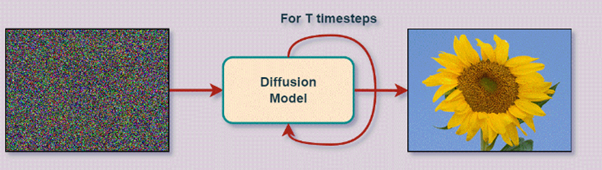
\includegraphics[width=1\linewidth]{diff_iter.png}
    \caption{Диффузионный итеративный процесс восстановления фотографии из шума}
    \label{func::diff}
\end{figure}

Идея, используемая в неравновесной статистической физике, заключается в том, что мы можем постепенно преобразовывать одно распределение в другое.

Структура (распределение) исходного изображения постепенно 
разрушается путем добавления шума, а затем с использованием модели 
нейронной сети для восстановления изображения. Выполняя это достаточное количество раз и с хорошими данными, модель в итоге научится оценивать базовое (исходное) распределение данных. Затем мы можем просто начать с простого шума и использовать обученную нейронную сеть для создания нового изображения, представляющего исходный обучающий набор данных.

Опишем общую концепцию обучения:

\begin{enumerate_num}
    \item Берём начальное изображение.
    \item Итеративно добавляем Гауссовский шум, пока от исходного ничего не останется, только каша из пикселей.
    \item Обучаем модель шумоподавления приводить эту шум к результату, 
похожему на исходное изображение.
\end{enumerate_num}

Процесс прямого распространения:

\begin{enumerate_num}
    \item Исходное изображение медленно итеративно искажается (цепочка Маркова) путем добавления масштабированного гауссова шума.
    \item Этот процесс выполняется для некоторых временных шагов t, t + 1, t + 2 + ... + t + n.
    \item Изображение на временном шаге t создается из x(t - 1) + шум.
    \item На этом этапе модель не задействована.
    \item В конце этапа прямой диффузии xt, из-за итеративного добавления шума, мы остаемся с чистым зашумленным изображением, представляющим <<изотропный гауссовский>>. Это просто математический способ сказать, что у нас есть стандартное нормальное распределение, и дисперсия распределения одинакова по всем измерениям. Мы преобразовали распределение данных в гауссово распределение   
\end{enumerate_num}

Процесс обратного распространения(обратная диффузия):

\begin{enumerate_num}
    \item  На этом этапе мы отменяем процесс пересылки. Задача состоит в том, чтобы удалить шум, добавленный в прямом процессе, снова итеративным способом (цепочка Маркова). Это делается с использованием модели нейронной сети.
    \item Задача модели заключается в следующем: учитывая временной интервал t и зашумленное изображение xt, необходимо спрогнозировать шум, добавленный к изображению на шаге t - 1.
    \item Модель предсказывает (аппроксимирует) шум, добавленный к xt - 1 при прямом проходе.
\end{enumerate_num}

Если сравнивать Сравнение GAN и Диффузионной модели, то оба генеративных алгоритма GAN и метод генерации изображений с помощью диффузионных моделей позволяют генерировать новые данные, однако в них все же есть некоторые отличия:

\begin{enumerate_num}
    \item  Из-за итеративного характера процесса распространения процесс обучения и генерации у диффузионных моделей, как правило, более стабилен, чем GAN.
    \item В GAN модель генератора должна перейти от чистого шума к изображению за один шаг xt → x0, что является одним из источников нестабильного обучения.
    \item В отличие от GAN, где для обучения требуются две модели, в диффузиях требуется только одна модель.
\end{enumerate_num}

Одно из наблюдений из приведенного выше изображения заключается в том, что размер изображения остается неизменным на протяжении всего процесса, в отличие от GAN, где скрытый тензор может иметь разные размеры. Это может быть проблемой при создании высококачественных изображений из-за ограниченной памяти графического процессора. Однако авторы <<Стабильной диффузии>> (точнее, <<скрытой диффузии>>) обходят эту проблему, используя вариационный автоэнкодер.

Для ускорения процесса генерации изображений  диффузионные модели выполняет процесс диффузии не с самими пиксельными изображениями, а со сжатой версией изображения, также это называется «переходом в скрытое пространство».

Это сжатие (и последующая распаковка/рисование) выполняется при помощи автокодировщика, принцип работы которого представлен на рисунке~\ref{func::coder}. Автокодировщик сжимает изображение в скрытое пространство(latent) при помощи своего кодировщика, а затем воссоздаёт его при помощи декодера на основе только сжатой информации

\begin{figure}[ht]
    \centering
    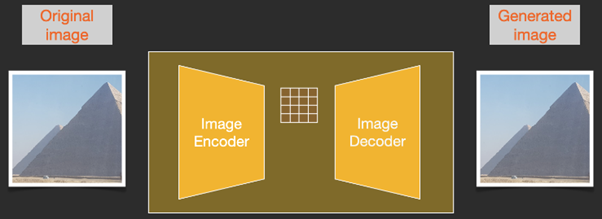
\includegraphics[width=.9\linewidth]{coder.png}
    \caption{Принцип работы кодировщика}
    \label{func::coder}
\end{figure}

Далее со сжатыми latent выполняется прямой процесс диффузии. Используются срезы шума, применяемые к этим latent, а не к пиксельному изображению. То есть предсказатель шума на самом деле обучается прогнозировать шум в сжатом описании (в скрытом пространстве).

При помощи прямого процесса (с использованием кодировщика автокодировщика) мы генерируем данные для обучения предсказателя шума. После его обучения мы можем генерировать изображения, выполняя обратный процесс (при помощи декодера автокодировщика) как показано на рисунке~\ref{func::diff_proc}.

\begin{figure}[ht]
    \centering
    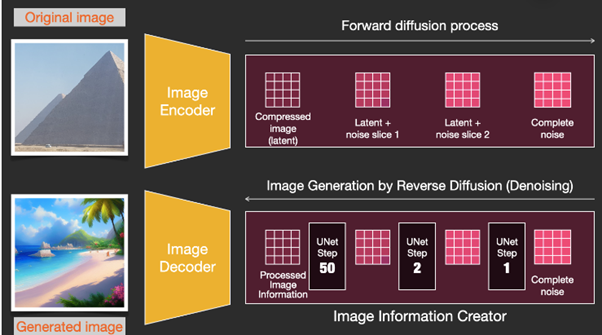
\includegraphics[width=.75\linewidth]{diff_proc.png}
    \caption{Процесс прямой и обратной диффузии}
    \label{func::diff_proc}
\end{figure}

Упрощенная схема диффузионной модели, которая способа обрабатывать текстовый ввод можно увидеть на рисунке~\ref{func::diff_simple}

\begin{figure}[ht]
    \centering
    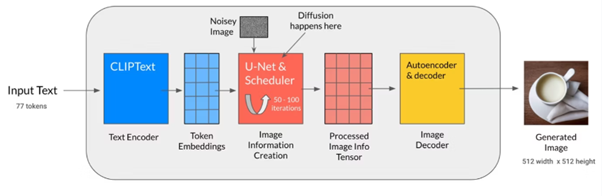
\includegraphics[width=0.9\linewidth]{diff_simple.png}
    \caption{Упрощенная схема диффузионной модели}
    \label{func::diff_simple}
\end{figure}

\subsection{Блок обработки текста}

Языковая модель Transformer используется в качестве компонента понимания языка, она получает текстовую строку и создаёт эмбеддинги токенов. В опубликованной диффузионной модели используется ClipText – модель на основе GPT~\cite{gpt}. Как показывает практика выбор языковой модели очень важен. Замена на более объёмные языковые модели сильнее влияет на качество генерируемого изображения, чем более объёмные компоненты генерации изображений.

В первых диффузионных моделях просто подключалась предварительно обученная модель ClipText, выпущенная OpenAI. Возможно, будущие модели перейдут на новые и гораздо более объёмные OpenCLIP-варианты CLIP. В эту новую группу входных векторов включены текстовые модели размерами до 354 миллионов параметров, в отличие от 63 миллионов параметров в ClipText.

CLIP обучается на массиве изображений и подписей к ним. Массив данных выглядит примерно так как показано на рисунке~\ref{func::clip_lern_data}, только состоит из 400 миллионов изображений и подписей

\begin{figure}[ht]
    \centering
    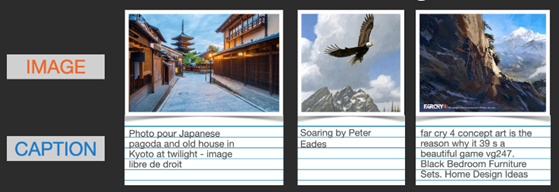
\includegraphics[width=.9\linewidth]{clip_lern_data.png}
    \caption{Пример данных для обучения текстовой модели CLIP}
    \label{func::clip_lern_data}
\end{figure}

CLIP~-- это сочетание кодировщика изображений и кодировщика текста. Обучающий процесс модели, приведенный на рисунке~\ref{func::clip_lern}, можно упрощённо представить как кодирование изображения и его подписи кодировщиками изображений и текста.

\begin{figure}[ht]
    \centering
    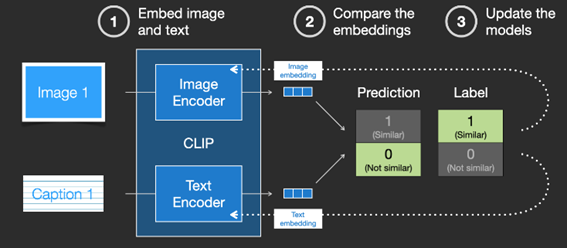
\includegraphics[width=.7\linewidth]{clip_lern.png}
    \caption{Обучающий процесс текстовой модели CLIP}
    \label{func::clip_lern}
\end{figure}

Затем мы сравниваем получившиеся эмбеддинги при помощи косинусного коэффициента. В начале процесса обучения схожесть будет низкой, даже если тест описывает изображение правильно.

Мы обновляем две модели так, чтобы в следующий раз при создании эмбеддингов получившиеся эмбеддинги были схожими. Повторяя этот процесс со всем массивом данных и группами входных векторов большого размера, мы получаем кодировщики, способные создавать эмбеддинги, в которых изображение собаки и предложение <<a picture of a dog>> схожи. Как и в word2vec, процесс обучения также должен включать в себя отрицательные примеры изображений и подписей, которые не совпадают, а модель должна присваивать им низкую оценку схожести.

\subsection{Блок обработки данных для диффузионной модели}

Чтобы сделать текст частью процесса генерации изображений, нам нужно модифицировать предсказатель шума так, чтобы он использовал в качестве входных данных текст.

Для начала рассмотрим диффузионную U-Net, не использующую текст. Её входы и выходы выглядят как показано на рисунке~\ref{func::unet_base}.

\begin{figure}[ht]
    \centering
    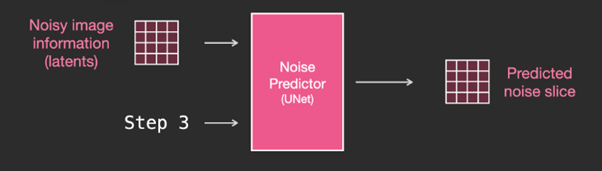
\includegraphics[width=.8\linewidth]{unet_base.png}
    \caption{Диффузионная модель  U-Net, не использующая текст}
    \label{func::unet_base}
\end{figure}

U-Net~-- это последовательность слоёв, работающая над преобразованием массива latent. Каждый слой модели обрабатывает выходные данные предыдущего слоя. Часто выходных данных подается (через остаточные соединения) для обработки на дальнейших этапах сети. Шаг времени преобразуется в вектор эмбеддингов шага времени, который используется в слоях.

Теперь рассмотрим слои предсказателя шума U-Net с текстом или как изменить эту систему, чтобы уделить внимание тексту. Основное изменение системы, которое необходимо для добавления поддержки текстового ввода~-- добавление слоя attention между блоками ResNet. Измененная модель с блоками attention показана на рисунке~\ref{func::unet_changed}.

\begin{figure}[ht]
    \centering
    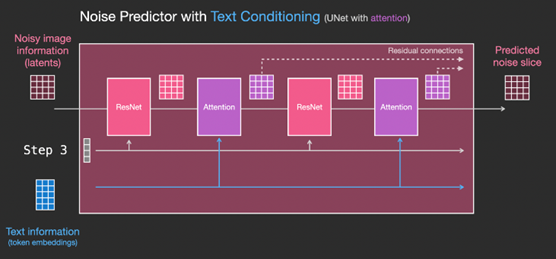
\includegraphics[width=0.9\linewidth]{unet_changed.png}
    \caption{Модель U-Net с блоками attention на текстовую информацию}
    \label{func::unet_changed}
\end{figure}

Как можно увидеть, блок ResNet не смотрит непосредственно на текст. Слои attention объединяют эти текстовые описания в latent. И теперь следующий ResNet может использовать эту встроенную текстовую информацию в своей обработке.

\subsection{Архитектура нейронной сети для сегментации}

U-Net считается одной из стандартных и основных архитектур CNN для задач сегментации изображений, когда нужно не только определить класс изображения целиком, но и сегментировать его области по классу, т. е. создать маску, которая будет разделять изображение на несколько классов. Особое применение данной нейросети используется в медицине, где количество размеченных данных очень мало, пример работы сети U-Net представлен на рисунке~\ref{func::unet}.  

Для U-Net характерно:
\begin{enumerate_num}
    \item Достижение высоких результатов в различных реальных задачах, особенно для биомедицинских приложений.
    \item Использование небольшого количества данных для достижения хороших результатов.
\end{enumerate_num}


\begin{figure}[ht]
    \centering
    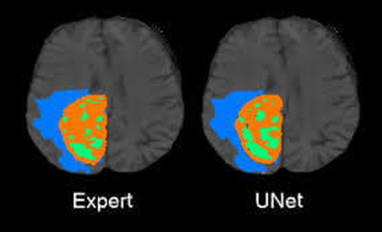
\includegraphics[width=0.89\linewidth]{unet.png}
    \caption{Сравнение сегментации отделов головного мозга нейронной сетью U-Net и ручной разметкой экспертного врача}
    \label{func::unet}
\end{figure}

Архитектура состоит из стягивающего пути для захвата контекста и симметричного расширяющегося пути, который позволяет осуществить точную локализацию. 
Сеть обучается сквозным способом на небольшом количестве изображений. U-Net заняла первое место в конкурсе ISBI 2015 года по трекингу клеток. Кроме того, эта сеть работает быстро. Сегментация изображения 512×512 занимает менее секунды на современном графическом процессоре.

Архитектура сети приведена на рисунке~\ref{func::unet_arch}. Каждый синий квадрат соответствует многоканальной карте свойств. Количество каналов приведено в верхней части квадрата. Размер x-y приведен в нижнем левом краю квадрата. Белые квадраты представляют собой копии карты свойств. Стрелки обозначают различные операции. Нейронная сеть U-Net представляет собой последовательность слоёв свёртка+пулинг, которые сначала уменьшают пространственное разрешение картинки, а потом увеличивают его, предварительно объединив с данными картинки и пропустив через другие слои свёртки. Таким образом, сеть выполняет роль своеобразного фильтра. Она состоит из сужающегося пути (слева) и расширяющегося пути (справа). Сужающийся путь – типичная архитектуре сверточной нейронной сети. Он состоит из повторного применения двух сверток 3×3, за которыми следуют ReLU и операция максимального объединения (2×2 степени 2) для понижения разрешения.

\begin{figure}[ht]
    \centering
    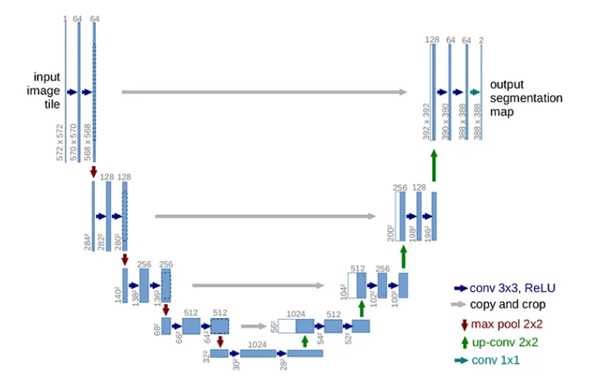
\includegraphics[width=0.9\linewidth]{unet_arch.png}
    \caption{Архитектура U-Net}
    \label{func::unet_arch}
\end{figure}

На каждом этапе понижающей дискретизации каналы свойств удваиваются. Каждый шаг в расширяющемся пути состоит из операции повышающей дискретизации карты свойств, за которой следуют:
\begin{enumerate_num}
    \item Свертка 2×2, которая уменьшает количество каналов свойств.
    \item Объединение с соответствующим образом обрезанной картой свойств из стягивающегося пути.
    \item Две 3×3 свертки, за которыми следует ReLU.
\end{enumerate_num}

На последнем слое используется свертка 1×1 для сопоставления каждого 64-компонентного вектора свойств с желаемым количеством классов. Всего сеть содержит 23 сверточных слоя.

После сегментации изображения на выходе образуется одноканальное бинарное изображение, которое сравнивается с поданной соответствующей сегментируемому изображению маской. Сравнение происходит с целью определения ошибки, допускаемой моделью, в ходе сегментации поданного на вход модели изображения. Определение ошибки производится на основе вычисленного значения несовпадения одноканальных изображений, таких как предсказание модели и соответствующая данному предсказанию маска, по каждому пикселю. Примерами таких методов могут послужить мера сходства Жаккара, коэффициент Сёренсена, функции ошибки бинарная кросс-энтропия и метод наименьших квадратов.
